\documentclass[reprint, amsmath, amssymb, floatfix, aps, pra]{revtex4-2}

\usepackage{bm}
\usepackage{graphicx}
\usepackage{hyperref}
\usepackage[ruled, vlined]{algorithm2e}
\usepackage{qcircuit}
\usepackage[caption=false]{subfig}
\newcommand{\ket}[1]{|#1\rangle}
\newcommand{\bra}[1]{\langle #1 |}
\newcommand{\braket}[3][2]{\langle #2|#3 \rangle}

\graphicspath{{./assets/figures/}}

\begin{document}

\preprint{}

\title{Long-range intermolecular interactions on a continuous-variable quantum computer}

\author{Matthieu Sarkis}
\email{matthieu.sarkis@uni.lu}
\affiliation{
Department of Physics and Materials Science\\ University of Luxembourg, L-1511, Luxembourg City, Luxembourg.
}

\author{Alessio Fallani}
\email{alessio.fallani@uni.lu}
\affiliation{
Department of Physics and Materials Science\\ University of Luxembourg, L-1511, Luxembourg City, Luxembourg.
}

%\author{Alexandre Tkatchenko}
%\email{alexandre.tkatchenko@uni.lu}
%\affiliation{
%Department of Physics and Materials Science\\ University of Luxembourg, L-1511, Luxembourg City, Luxembourg.
%}

\date{\today}

\begin{abstract}
    We study the full Coulomb Quantum Drude Oscillator model for intermolecular dispersion interactions using a continuous-variable instance of the Variational Quantum Eigensolver algorithm. Being bosonic in nature, the Quantum Drude Oscillator model indeed lends itself naturally to simulation on a photonic quantum computer, and we successfully reproduce in particular the binding energy curve profile of diatomic systems leveraging on Xanadu's open source Strawberry Field photonics library. We finally make some observations about the behavior of the entanglement entropy of the system in regards to the formation of bound states.
\end{abstract}

\keywords{Continous variable quantum computing, dispersion interactions}

\maketitle

%\tableofcontents

\paragraph*{Introduction}

    Van der Waals forces originate from the electromagnetic interaction between electrically neutral atoms or molecules \cite{margenau2013theory,kaplan2006intermolecular,stone2013theory,hirschfelder2009intermolecular} and arise from the coupling of matter to the background quantum eletrodynamic gauge field \cite{casimir1948influence,buhmann2013dispersion,buhmann2007dispersion,compagno1995atom,passante2018dispersion, cohen1997photons,cohen1998atom,bookpreparata,salam2009molecular,craig1998t}. Dispersion forces are critical to describe the properties of macromolecules such as their structure \cite{hoja2019reliable}, stability \cite{hoja2018first,mortazavi2018structure}, dynamics \cite{stohr2019quantum,reilly2014role,galante2021anisotropic} and response properties to electromagnetic signals \cite{kleshchonok2018tailoring, ambrosetti2022optical} and coupling to a background gauge field \cite{Karimpour_2022, karimpour2021comprehensive}. The inclusion of dispersion interactions can be done in an economical way by means of many-body methods \cite{richardson1975dispersion,mahanty1973dispersion,woods2016materials,tkatchenko2015current,ren2012random,harl2009accurate,dobson2012calculation,parsegian2005van,becke2006simple,becke2006exchange,grimme2010consistent,grimme2006semiempirical,tkatchenko2012accurate,massa2021many}, in particular through the so-called Many-Body Dispersion (MBD) framework, whose accuracy was proven in the litterature \cite{tkatchenko2012accurate,ambrosetti2014long}. In the MBD framework, drawing inspiration from the Drude atomic model, the response of valence electrons in atoms is assumed to be linear and this can be implemented through the introduction of Quantum Drude Oscillators (QDO). By assimilating the atom to a point particle (called Drudon) of mass $m$ and electric charge $-q$ attached to a fixed (in a Born-Oppenheimer fashion) nucleus of charge $+q$ by a harmonic spring characterized by a frequency $\omega$, QDOs define a compact coarse-grained quantum-mechanical model for dispersion forces. Molecules are then defined as a collection of QDOs interacting through \textit{dipole-dipole interaction} \cite{doi:10.1063/1.1743992, doi:10.1063/1.1743991}. Though simple, through a numerical treatment this system was shown to capture long-range phenomena in large biomolecular systems \cite{https://doi.org/10.48550/arxiv.2205.11549}. By construction, the MBD framework relies on the dipole-dipole approximation to the Coulomb interaction, and therefore comes at the cost of limiting the allowed range of interatomic distances (due to the finiteness of the multipolar expansion radius of convergence), and of leaving aside any contribution coming from high-order terms. These limitations can be addressed via multipolar generalizations of the pairwise second-order perturbative approaches \cite{massa2021beyond,massa2021many,becke2006simple,becke2006exchange}.

    In this Letter we propose, in the spirit of the Full Configuration Interaction (FCI) approach of \cite{sadhukhan2016quantum}, to study the MBD model with full Coulomb interaction between its constituents. The reader will find in fig. \ref{fig:qdos} a cartoon picture of a full-Coulomb two-QDO system.

    \begin{figure}
        %\hspace{1.25cm}
        %\begin{subfigure}
        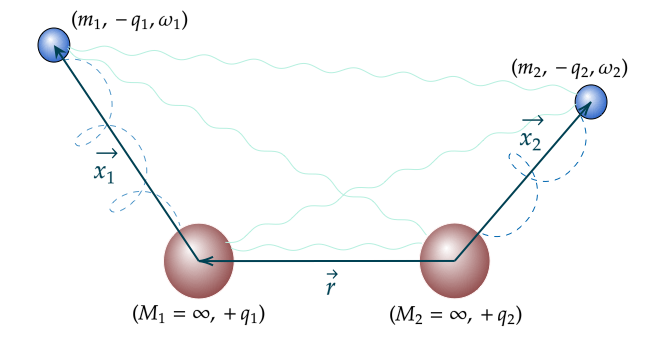
\includegraphics[scale=0.35]{figures/qdos.png}
        %\end{subfigure}
        \caption{\label{fig:qdos}Illustration of a system composed of a pair of QDOs. The nuclei are considered to be infinitely massive. The drudons interact with their nucleus through a harmonic potential, but with the other QDO through Coulomb interaction. $\bm x_i$ denote the relative position of the drudon with respect to its nucleus in QDO $i$. $\bm r$ denotes the position of $\text{QDO}_1$ with respect to $\text{QDO}_2$.}
    \end{figure}

    The main purpose of this Letter is to probe the use of NISQ quantum computing algorithms to the study of concrete quantum chemistry models, beyond the standard electronic structure problem of small molecules \cite{peruzzo2014variational, kandala2017hardware, nam2020ground}. Similar work has appeared recently in \cite{anderson2022coarse} in which the authors implement a Variational Quantum Eigensolver for the simulation of an effective one-dimensional QDO model and run it on IBM's superconducting qubit device. There, the quantum harmonic oscillator Hilbert space is truncated at some fixed level $\Lambda$, and mapped to the Hilbert space of a system of $\lceil\log_2\Lambda\rceil$ qubits. Instead here, the choice of photonics-based quantum computing paradigm is guided by the intrinsic bosonic nature of quantum Drude oscillator, therefore effectively mapping a bosonic problem onto a bosonic hardware. The Fock space of a single harmonic oscillator is directly identified with the Fock space of one mode (one photon channel, in quantum optics language) of the quantum electrodynamic gauge field. In particular, the position and momentum of the drudon particle are directly identified with the position and momentum quadratures of the electromagnetic field. In other words, the continous-variable quantum computing paradigm \cite{lloyd1999quantum, pati2000quantum, pati2003deutsch, braunstein2005quantum, andersen2010continuous, lomonaco2002continuous, zhong2020quantum, tillmann2013experimental} is adopted, and a collection of $N$ quantum Drude oscillators is then represented by a collection of $N$ photon channels in an optical circuit. Similar ideas were successfully used to simulate bosonic Euclidean quantum fields \cite{marshall2015quantum, yeter2022quantum} on a lattice. Concerning the quantum simulation of interacting harmonic oscillators in a first quantized framework, let us mention \cite{Culver:2021rxo}, where the authors encode simple supersymmetric quantum mechanical systems into a system of qubits, using again a hard cutoff for the bosonic degrees of freedom. In our case, and following  \cite{schuld2021machine, killoran2019continuous, arrazola2019machine, enomoto2022continuous, peruzzo2014variational}, an optical circuit is composed of parameterized linear gates like beam-splitters, phase shifters, but also Gaussian gates implementing displacement and squeezing, and quartic gates (Kerr gates). A VQE type algorithm is then applied to optimize the parameters of the ciruit for preparation of the ground state wavefunction of the quantum Drude Oscillator system. For the implementation, we leverage on Xanadu's Strawberry Fields quantum machine learning framework for continuous-variable hybrid quantum-classical optimization \cite{schuld2021machine, killoran2019continuous, arrazola2019machine, bromley2020applications}. Following the work \cite{arrazola2019machine} for state preparation, we probe our approach using Strawberry Fields simulator.
    Even though we are focusing on dispersion, long-range intermolecular interactions in this Letter, let us mention among other successful applications of quantum computing to study molecular spectra, binding energy curve, molecular force fields and ground state preparation exist in the litterature \cite{kiss2022quantum, apanavicius2021morse, wang2009efficient, nam2020ground, romero2018strategies, colless2018computation, kandala2017hardware}.
    \newline
\paragraph*{Definition of model}

        The Hamiltonian describing a system of $N$ Quantum Drude Oscillators in three dimensions is given by:
        \begin{equation*}
            H=\sum_{i=1}^N\left[\frac{\bm{p} _i^2}{2m_i} + \frac{1}{2}m_i\omega_i^2\bm{x} _i^2\right] +\sum_{i<j}V_\text{Coul}\left(\bm{x} _i, \bm{x} _j\right)\,,
        \end{equation*}
        with the Coulomb interaction receiving contributions from interacting drudon-drudon and drudon-nucleus pairs:
        \begin{equation*}
        \begin{split}
            \frac{V_\text{Coul}\left(\bm{x} _i, \bm{x} _j\right)}{q_iq_j}=&\ \frac{1}{r_{ij}} - \frac{1}{|\bm{r}_{ij}
            + \bm{x} _i|} - \frac{1}{|\bm{r}_{ij}  - \bm{x} _j|} \\
            & + \frac{1}{|\bm{r}_{ij} - \bm{x} _j + \bm{x} _i|}\,,
        \end{split}
        \end{equation*}
        and where $\bm x_i$ denotes the relative position of drudon $i$ with respect to its nucleus. The usual approach consists in solving the theory in the multipolar expansion framework, in which the potential can be expressed as a power series in the inverse distance separating the two nuclei:
        \begin{equation*}
            V_\text{Coul}\left(\bm{x} _i, \bm{x} _j\right)= \sum_{n\geq 0} V_n\left(\bm{x} _i, \bm{x} _j\right)\,,
        \end{equation*}
        with the following scaling behavior $V_n\left(\bm{x} _i, \bm{x} _j\right)\propto r_{ij}^{-n-3}$.
        The potential $V_0$ corresponds then to the dipole-dipole interaction, and is at the core of the Many Body Dispersion (MBD) model. $V_1$ corresponds to the dipole-quadrupole interaction, and $V_2$ to the quadrupole-quadrupole and dipole-octupole interaction.

        One obvious limitation of the multipolar expansion is the lower bound it imposes on the interatomic distance. One can easily see that within the MBD (dipole-dipole) model by direct diagonalization of the quadratic Hamiltonian in terms of normal modes. In that case, one of the normal modes (the center of mass mode) develops a purely imaginary frequency at short range. Higher order physical effects are also neglected in the MBD model, motivating the study of the QDO model with full Coulomb interaction potential between its constituents.

        Let us define the following dimensionless position and momententum operators associated to QDO $i$:
        \begin{equation*}
            \bm{X}_i := \sqrt{\frac{m_i\omega_i}{\hbar}}\,\bm{x}_i\,,\ \ \ \ \ \bm{P}_i := \frac{\bm{p}_i}{\sqrt{\hbar m_i\omega_i}}\,,
        \end{equation*}
        in terms of which the Hamiltonian reads
        \begin{equation*}
        \begin{split}
            H =&\ \sum_{i=1}^N\frac{\hbar\omega_i}{2}\left(\bm X_{i}^2 + \bm P_{i}^2\right) \\
            & + \sum_{i<j}V_\text{Coul}\left(\sqrt{\frac{\hbar}{m_i\omega_i}}\bm{X} _i, \sqrt{\frac{\hbar}{m_j\omega_j}}\bm{X} _j\right)\,.
        \end{split}
        \end{equation*}
        One can define the $3N$ creation and annihilation operators
        \begin{equation*}
            \bm a_{i} = \frac{\bm X_{i} + i\bm P_{i}}{\sqrt 2}\,,\ \ \ \ \ \bm a^\dagger_{i} = \frac{\bm X_{i} - i\bm P_{i}}{\sqrt 2}\,,
        \end{equation*}
        in terms of which the Hamiltonian reads
        \begin{equation*}
        \begin{split}
            &H = \sum_{i=1}^N\hbar\omega_i\left(\bm a_{i}^\dagger\cdot\bm a_{i} +\frac{3}{2}\right) \\
            & + \sum_{i<j}V_\text{Coul}\left(\sqrt{\frac{\hbar}{m_i\omega_i}}\frac{\bm a_i + \bm a_i^\dagger}{\sqrt 2}, \sqrt{\frac{\hbar}{m_j\omega_j}}\frac{\bm a_j + \bm a_j^\dagger}{\sqrt 2}\right)\,.
        \end{split}
        \end{equation*}
        Let us from now on restrict the problem to a pair of QDOs ($N=2$) for concreteness, though the following developements carry to bigger systems. We denote by $d$ the interatomic distance.

        In order to reduce the complexity of the problem, let us define one-dimensional instances of the QDO model as follows: we restrict the movement of the two drudons to be along a common axis (directed by a unit vector $\hat{\bm e}_\theta$) which form an angle $\theta\in[0,\pi/2]$ with respect to the vector $\bm r_{12}$ connecting the two nuclei. We therefore have a family of one-dimensional models which can be obtained from the full-fledged 3d model simply by setting to zero the contribution from the oscillator modes belonging to the plane perpendicular to $\hat{\bm e}_\theta$. Let us denote by $(X, P)$ the remaining position and momentum degree of freedoms. As limiting cases, we obtain models in which the drudons are constrained to move either in the direction parallel to the axis separating the two nuclei ($\theta=0$), or perpendicular to the latter ($\theta=\pi/2$). Those two models were studied in \cite{anderson2022coarse} in the dipole-dipole approximation. As mentioned in the introduction, in that paper the authors encode the states in the truncated Fock space of the system into the state of a set of qubits, and run VQE-type algorithms on IBQ quantum processors. However as we will see, the angle $\theta$ captures the competition between \textit{existence of binding} (for small $\theta$) and \textit{smoothness} (for large $\theta$), and interesting one-dimensional models actually sit at values of $\theta$ in the open segment $(0,\pi/2)$.

        In the case of a generic angle $\theta$ and interatomic distance $d$, the one-dimensional Coulomb potential reads:
        \begin{equation*}
        \begin{split}
            &\frac{V_\text{Coul}^{\theta, d}(x_1, x_2)}{q_1q_2} = \frac{1}{d} - \frac{1}{\sqrt{d^2+2d(\cos\theta) x_1+x_1^2}} \\
            &- \frac{1}{\sqrt{d^2-2d(\cos\theta) x_2+x_2^2}} \\
            &+\frac{1}{\sqrt{d^2 - 2d(\cos\theta) (x_2-x_1) + (x_2-x_1)^2}}\,.
        \end{split}
        \end{equation*}
        We therefore have a family of Hamiltonians parameterized by $(\theta, d)\in[0, \pi/2]\times\mathbb R_{>0}$:
        \begin{equation}
        \label{eq:finalHamiltonian}
        \begin{split}
            H_{\theta, d}=&\ \frac{\hbar\omega_1}{2}\left(P_1^2 + X_1^2\right) + \frac{\hbar\omega_2}{2}\left(P_2^2 + X_2^2\right)\\
            &+V_\text{Coul}^{\theta, d}\left(\sqrt{\frac{\hbar}{m_1\omega_1}}X_1, \sqrt{\frac{\hbar}{m_2\omega_2}}X_2\right)\,.
        \end{split}
        \end{equation}
        Alternatively, in terms of creation and annihilation operators, one has
        \begin{equation}
        \label{eq:Hamiltonian_heterodyne}
        \begin{split}
            H_{\theta, d} &= \hbar\omega_1\left( a_{1}^\dagger a_{1} +\frac{1}{2}\right) + \hbar\omega_2\left(a_{2}^\dagger a_{2} +\frac{1}{2}\right) \\
            & + V_\text{Coul}^{\theta, d}\left(\sqrt{\frac{\hbar}{m_1\omega_1}}\frac{a_1 + a_1^\dagger}{\sqrt 2}, \sqrt{\frac{\hbar}{m_2\omega_2}}\frac{a_2 + a_2^\dagger}{\sqrt 2}\right)\,.
        \end{split}
        \end{equation}
        For the numerical simulations, we set $\hbar=4\pi\epsilon_0=1$ as well as $m_i=q_i=\omega_i=1$ for both QDOs.
\newline
\paragraph*{Photonic circuit and Variational Algorithm}

    From a molecular physics and long-range intermolecular perspective, we are mainly interested in knowing the ground state of the system (\ref{eq:finalHamiltonian}). Among the various approaches, the mixed quantum-classical variational algorithms were shown to be particularly efficient at capturing the properties of potentially complicated quantum states. Following \cite{killoran2019continuous, arrazola2019machine}, we apply a continuous-variable version of the variational quantum eigensolver algorithm to extract the ground state of the QDO system. The ground state is obtained by optimizing the parameters of a parameterized optical circuit composed of linear multi-modes gates (two-mode beamsplitters and rotation gates), Gaussian gates (single-mode squeezing and displacement gates), as well as non-Gaussian gates (Kerr gates) implementing non-linearity. Multiple layers constructed out of these gates are stacked to increase the complexity of the ansatz space, cf. fig. \ref{fig:quantum_circuit}.
    \begin{figure}
        \begin{equation*}
            \Qcircuit  @C=1em @R=1em {
            & \multigate{1}{BS}  & \gate{R}  & \gate{S}  & \multigate{1}{BS}  & \gate{R}  & \gate{D}  & \gate{K}  & \qw \gategroup{1}{5}{2}{6}{.7em}{--} \\
            & \ghost{BS}  & \qw  & \gate{S}  & \ghost{BS}  & \qw  & \gate{D}  & \gate{K} &
         \qw \gategroup{1}{2}{2}{3}{.7em}{--}
         \\
        }
        \end{equation*}
        \caption{\label{fig:quantum_circuit}One layer in the optical quantum circuit. The various gates, namely the beamsplitters, rotation, squeezing, displacement and Kerr gates are collectively parameterized by $\omega$.}
    \end{figure}
    In the procedure, the relative coordinate of the drudons with respect to their nucleus is directly identified with the position quadrature of the quantized electromagnetic field along the two channels of the optical quantum circuit.

    Overall, denoting by $\omega$ the set of all parameters, the circuit implements a unitary $U(\omega)$ acting on an input reference state that we simply take to be the Fock vacuum state $|0\rangle$. The state prepared by the circuit is therefore given by
    \begin{equation*}
        |\psi(\omega)\rangle = U(\omega)|0\rangle\,.
    \end{equation*}
    Once the ansatz state $|\psi(\omega)\rangle$ has been produced, one extracts the value of the energy in that state, given by
    \begin{equation*}
        \langle\psi(\omega)|H|\psi(\omega)\rangle\,.
    \end{equation*}
    Let us denote expectations in the state $|\psi(\omega)\rangle$ by angular brackets $\langle\cdot\rangle$.
    To be specific, let us take the model $H$, and let us denote by angular brackets the expectation in state $|\psi(\omega)\rangle$. One has
    \begin{equation}
    \label{eq:loss}
    \begin{split}
        \langle H\rangle =&\ \hbar\omega_1\left(\langle a_{1}^\dagger a_{1}\rangle+\frac{1}{2}\right)+\hbar\omega_2\left(\langle a_{2}^\dagger a_{2}\rangle+\frac{1}{2}\right)\\
        &+ \left\langle V_\text{Coul}^{\theta, d}\left(\sqrt{\frac{\hbar}{m_1\omega_1}} X_1, \sqrt{\frac{\hbar}{m_2\omega_2}} X_2\right)\right\rangle
    \end{split}
    \end{equation}
    by linearity of the expectation. On the second line one has to compute an expression of the form $\langle f(X_1, X_2)\rangle$. One therefore needs to extract the joint statistics of the position quadratures by preparation and measurements of the state $|\psi(\omega)\rangle$ in the quadrature basis, as summarized in alg. (\ref{alg:statistics_computation}). Once the joint probability density $\rho$ of $(X_1, X_2)$ in the state $|\psi(\omega)\rangle$ is known, one can compute
    \begin{equation*}
        \langle f(X_1, X_2)\rangle = \int_{\mathbb R^{6}}f(x_1, x_2)\rho(x_1, x_2)\,\text{d}x_1\text{d}x_2\,,
    \end{equation*}
    where the integral above should be understood a finite sum over a sufficiently refined grid $G_X\times G_X$ in the position quadratures plane. For the numerical simulation we take a linear grid $G_X$ composed of 500 points in the interval $[-6,6]$.

    Let us note that alternatively, and following \cite{arrazola2019machine}, the simulator of Strawberry Fields actually provides direct access to the output statevector expressed in the Fock basis:
    \begin{equation*}
        |\psi(\omega)\rangle = \sum_{n_1,n_2=0}^\infty \alpha_{n_1n_2}(\omega)|n_1\rangle\otimes|n_2\rangle\,.
    \end{equation*}
    The Fock space is actually truncated at a some fixed energy level, we choose that cutoff level to be 5. This choice of cutoff is not a real limitation and a larger value could be chosen instead, but 5 is sufficient, as was observed in particular using a FCI approach \cite{sadhukhan2016quantum}.
    The amplitude of a specific pair of the quadratures $(X_1, X_2)$ is then given by:
    \begin{equation*}
        \langle X_1,X_2|\psi(\omega)\rangle = \sum_{n_1,n_2=0}^\infty \alpha_{n_1n_2}(\omega)\prod_{i=1}^{2}\frac{e^{-\frac{X_i^2}{2}}H_{n_i}(X_i)}{\sqrt{\pi^{1/2}2^{n_i}n_i!}}\,,
    \end{equation*}
    in terms of the Hermite polynomials. The joint law of the quadratures in the state $|\psi(\omega)\rangle$ is therefore given by
    \begin{equation*}
        \rho(X_1,X_{2}) = \left|\langle X_1,X_2|\psi(\omega)\rangle\right|^2\,.
    \end{equation*}
    After extracting as well the mean photon numbers $\langle n_1\rangle$ and $\langle n_2\rangle$, one obtains $\langle H\rangle$.

    We then define the cost function
    \begin{equation}
    \label{eq:definition_cost}
        \mathcal C(\omega) := \langle\psi(\omega)|H|\psi(\omega)\rangle\,,
    \end{equation}
    and update the parameters $\omega$ of the optical circuit in order to minimize that cost. This is summarized in alg. (\ref{alg:training}).

    \begin{algorithm}
        \caption{Extract distribution of position quadratures}\label{alg:statistics_computation}
            \textbf{Parameters:} statevector $|\psi\rangle$, finite subset $\mathcal {G}\in\mathbb R$, shots $M\in\mathbb N$

            \KwResult{Probability distribution of $(X_1, X_2)$ in state $|\psi\rangle$ discretized over the grid $G_X\times G_X$}\

            \For{$m=1$ to $|\mathcal G|$}{
                Initialize $N_m \gets 0$;
            }
            \For{$j=1$ to $M$}{
            Measure the state $|\psi\rangle$ in the discretized position quadratures basis, obtain the eigenvalue $X_m$, set $N_m\gets N_m+1$\;
            }
            \For{$m=1$ to $|\mathcal G|$}{
                Normalize $N_m \gets N_m / M$;
            }
            \textbf{return} $\{N_m\}_{m=1}^M$.
    \end{algorithm}



    \begin{algorithm}
        \caption{Training of the parameterized photonic circuit}\label{alg:training}
        \textbf{Parameters:} Model $(\theta, d)$, $N_\text{steps}\in\mathbb N$, initial circuit parameters $\omega_0\in\mathbb R^K$, learning rate $\eta\in\mathbb R_+$

        \KwResult{Optimized hyperparameters $\omega\in\mathbb R^K$}\

        Initialize hyperparameters $\omega \gets \omega_0$\;
        \For{$i=1$ to $N_\text{steps}$}{
        Compute the loss $\mathcal C$ according to eq. (\ref{eq:definition_cost})\;
        Compute the gradient $\nabla_\omega\mathcal C$ with the shift rule\;
            Update the parameters $\omega \gets \omega - \eta\nabla_\omega\mathcal C$\;
        \textbf{end for}
        }
        \textbf{return} $\omega$.
    \end{algorithm}

    As a side remark, let us note that given the form of the Hamiltonian in terms of creation and annihilation operators (\ref{eq:Hamiltonian_heterodyne}), an alternative to the measurement of the position quadratures and photon number operators could be to perform a measurement in the coherent basis through heterodyne measurements.
    \newline

\paragraph*{Binding energy curve}

    We gather here the results of the simulations. We focus on the case of 2 QDOs. In particular we study the profile of the binding energy as a function of the distance between the two nuclei, and make a few observation about the behavior of the entanglement entropy of the system.

    We fix a grid $G_\theta\times G_d\subset [0, \pi/2]\times (0, 3.5]$, with $\text{card}(G_\theta)=20$ and $\text{card}(G_d)=200$. For each pair $(\theta, d)$ in the grid we perform the continuous-variables VQE algorithm to extract properties of the ground state of the Hamiltonian (\ref{eq:finalHamiltonian}). Let us denote by $|\psi_{\theta, d}\rangle$ the corresponding ground state.
    The binding energy is defined as the difference between the ground state energy of the system of interacting QDOs and the ground state energy of a system of uninteracting QDOs $H_0$, i.e. with electric charge turned off:
    \begin{equation*}
        E^\theta_b(d) = \langle\psi_{\theta, d}|H_{\theta, d}|\psi_{\theta, d}\rangle - \langle\psi_0|H_0|\psi_0\rangle
    \end{equation*}
    In fig. \ref{fig:binding} we report the binding energy curve, namely the value of the binding energy as a function of the interatomic distance $d$, for a fixed value of the angle $\theta$. We choose $\theta=0.58$ illustrating most of the results.

    \begin{figure}
        %\hspace{1.25cm}
        %\begin{subfigure}
        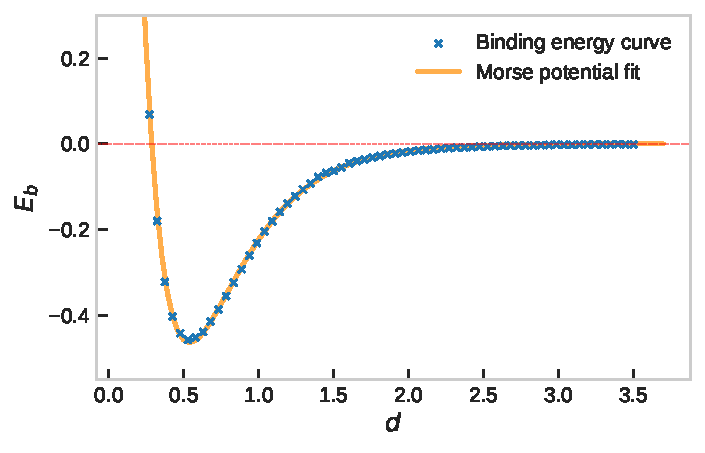
\includegraphics[scale=0.74]{figures/binding.pdf}
        %\end{subfigure}
        \caption{\label{fig:binding}Binding energy curve for the model at angle $\theta=0.58$, together with its Morse fit.}
    \end{figure}

    On fig. \ref{fig:binding} we observe a perfect agreement with a fit of Morse type \cite{herzberg1950spectra, apanavicius2021morse, le2006accurate, roy2007new, chiumorse2010}:
    \begin{equation}
    \label{eq:morse_fit}
        f(d) = E_b\left(e^{-2\frac{d-d_b}{s}} - 2e^{-\frac{d-d_b}{s}}\right)\,.
    \end{equation}
    The location of the bound state is given by $d_b\simeq 0.54$, with energy $-E_b\simeq 0.46$. The length scale $s$ is given by $s\simeq 2.75$. The quality of the Morse fit actully increases monotonically with the angle, cf. fig. \ref{fig:morse_quality}, the quality being defined by the $\ell^2$-distance between the numerical result and the fit.

    \begin{figure}
        %\hspace{1.25cm}
        %\begin{subfigure}
        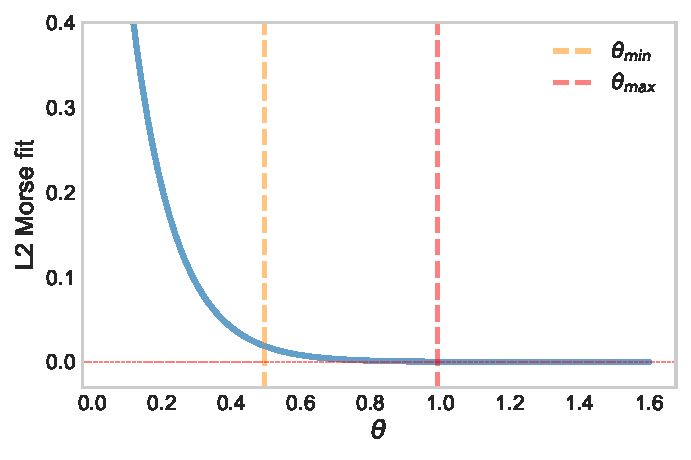
\includegraphics[scale=0.75]{figures/morse_quality.pdf}
        %\end{subfigure}
        \caption{\label{fig:morse_quality}\textbf{Blue curve:} Quality of the Morse fit as a function of the angle $\theta$, defined as the $\ell^2$-norm of the difference between the simulation and the Morse fit. \textbf{Yellow line:} Minimal angle above which the models are considered smooth. \textbf{Red line:} Maximal angle above which the models do not exhibit binding anymore.}
    \end{figure}

    By varying the value of the angle $\theta$, we observe two different regimes. For small values of the angle, the curve deviates more and more from a Morse curve, and in the extreme longitudinal case $\theta=0$, becomes highly non-smooth at short interatomic distances. This small angle regime is also characterized by the existence of a negative global minimum of the binding energy, hence by the existence of a bound state. On the other hand, as the angle increases, the $\ell^2$-quality of the fit becomes better. However, passed some value of the angle, the global minimum disappears together with the corresponding bound state. This competition between smoothness and existence of a bound state is illustrated in fig. \ref{fig:binding_vs_smooth}, and is of course signals of a phase transition of the model where $\theta$ plays the role of control parameter. Below a critical value $\theta_\star$ of the order parameter, the system is characterized by the existence of a bound state, which disappear above the critical value of $\theta_\star$.

    \begin{figure}
        %\hspace{1.25cm}
        %\begin{subfigure}
        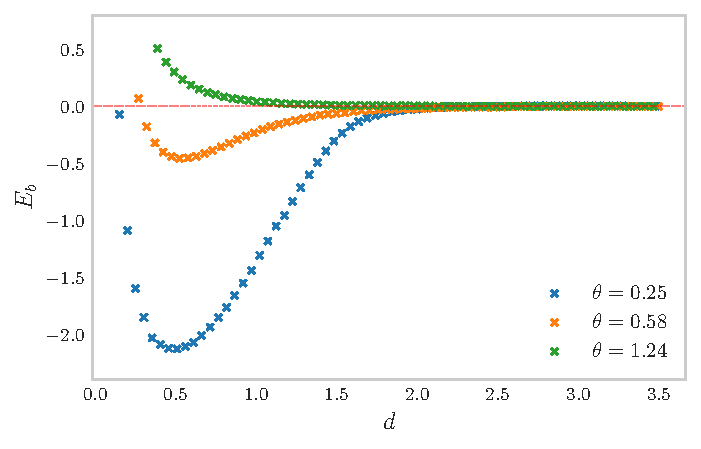
\includegraphics[scale=0.75]{figures/binding_vs_smooth.pdf}
        %\end{subfigure}
        \caption{\label{fig:binding_vs_smooth}Binding energy curve for three different values of the angle $\theta$ illustrating the tension between models close to $\theta=0$ and models close to $\theta=\pi/2$. For small angle (blue curve),  the strong curvature prevents a good Morse fit, while for large angle (green curve), the transverse configuration of the drudons prevents formation of a bound state. The orange curve corresponds an intermediate angle exhibiting both binding and an excellent Morse fit.}
    \end{figure}

    Both regimes can be understood physically as follows: for very small angle $\theta\ll \theta_\star$, and in particular for the longitudinal model $\theta=0$, as the two QDOs are getting closer and closer to each other, unstable configurations in which the two drudons are getting arbitrarily close to each other start appearing. Indeed, space being 1-dimensional and the two drudons moving along a common axis, as the two drudons get close to one another, the associated Coulomb repulsion component of the ground state energy diverges. On the other hand, for large angle $\theta\gg \theta_\star$, and \textit{a fortiori} for the transverse model $\theta=\pi/2$, two main configurations of the drudons may occur (thinking classically) depending on the relative position of the drudons with respect to the axis connecting the two nuclei. In the first configuration, the drudons are sitting on opposite sides. In that case, the dominant contribution to the energy between the two QDOs is the Coulomb repulsion between the nuclei. In the second configuration, the drudons are on the same side. In that case, in adding to the repulsive force between the two nuclei, one can also add up the repulsion force between the two drudons, leading to an even more repulsive scenario. Summing up, no binding can occur at $\theta=\pi/2$, and by smoothness of the binding energy as a function of $\theta$, this should also be the case in an open neighborhood of $\theta=\pi/2$.

    The above observation suggests the following recipe. The longitudinal model predict the existence of negative minima of the binding energy curve. It is however unstable due to the configurations of superposed drudons, as explained above. One can then \textit{regularize} this 1d model by allowing for a non-zero angle $\theta$, and slightly increase it until reaching a certain level of smoothness, that we have chosen here to be quantified by the quality of a Morse fit. The angle should however not be too large, smaller than the transition point beyond which the bound state disappears. This procedure defines a small range of models characterized by an angle $\theta\in[\theta_\text{min}, \theta_\text{max}]$, as illustrated on fig. \ref{fig:morse_quality}. Finally, the QDO parameters are to be tuned to match \textit{ab initio} computations for the two-body system of interest.

    \paragraph*{Phase space representation}
    In fig. \ref{fig:wigners_joint}, we provide two representations of the system at different values of the interatomic distance. On the left side, from top to bottom, we represent the marginal Wigner function of each of the two QDOs for closer and closer distances. At large distance $d=3.16$, the two QDOs are far apart and do not feel each other. This can be seen by the fact that the marginal Wigner functions are characteristic of purely Gaussian states. At distance $d=1.36$, the two QDOs start feeling each other's presence. This is illustrated by the two marginal Wigner functions starting to be elongated, mostly along the position quadrature axis. Distance $d=0.82$ corresponds to the distance of maximal entanglement entropy. We observe in that case that the marginal Wigner functions are characterized by a significant spread in both position and momentum quadrature directions. Finally, at the bound state distance $d=0.54$, the marginal Wigner functions appear to be mostly elongated along the momentum quadrature axis. This is clear since even though the configuration of the system has reached stability,characterized by the fact that the Wigner functions suggest a fairly neat localization of the drudons in space, the drudons being really close to each other lead to an increase in the spread of the momentum density. Observe also the appearance of regions of negativity of the partial Wigner functions, signature of the non-classicality of the state of the system \cite{Chabaud:2021pnh}, and witness of the entanglement in bipartite states \cite{arkhipov2018negativity}. The right column of fig. \ref{fig:wigners_joint} instead illustrates the joint probability distribution of the position quadratures. We observe again a Gaussian behavior at large distances, as it should for two independent harmonic oscillators, a maximal sqeezing at the maximal entanglement entropy point, and a more localized appearance at the bound state distance. Let us mention that a refined analysis around the distance of maximal position quadrature density spread, the unimodal joint position quadrature probability distribution develops a bimodal profile, with maximum of the original mode located around the origin (both drudons being in expectation centered at the locus of their respective nucleus), and maximum of the newly appeared mode shifted away from the origin. This bimodal feature of the joint position quadrature density, signature of tunneling, is very easily observable for a smaller angle theta, as can be seen on fig. \ref{fig:classical_potential_small_angle}, which is consistent of the large curvature, at the corresponding range of distances, of the binding curve for such small angles. After tunneling, the mode initially centered at the origin disappears, and remains only the shifted mode describing a stable bound state configuration in which each of the QDOs has developed a non-zero expected dipole moment, oriented in opposite directions.
    \newline

    \begin{figure*}
        %\hspace{1.25cm}
        %\begin{subfigure}
        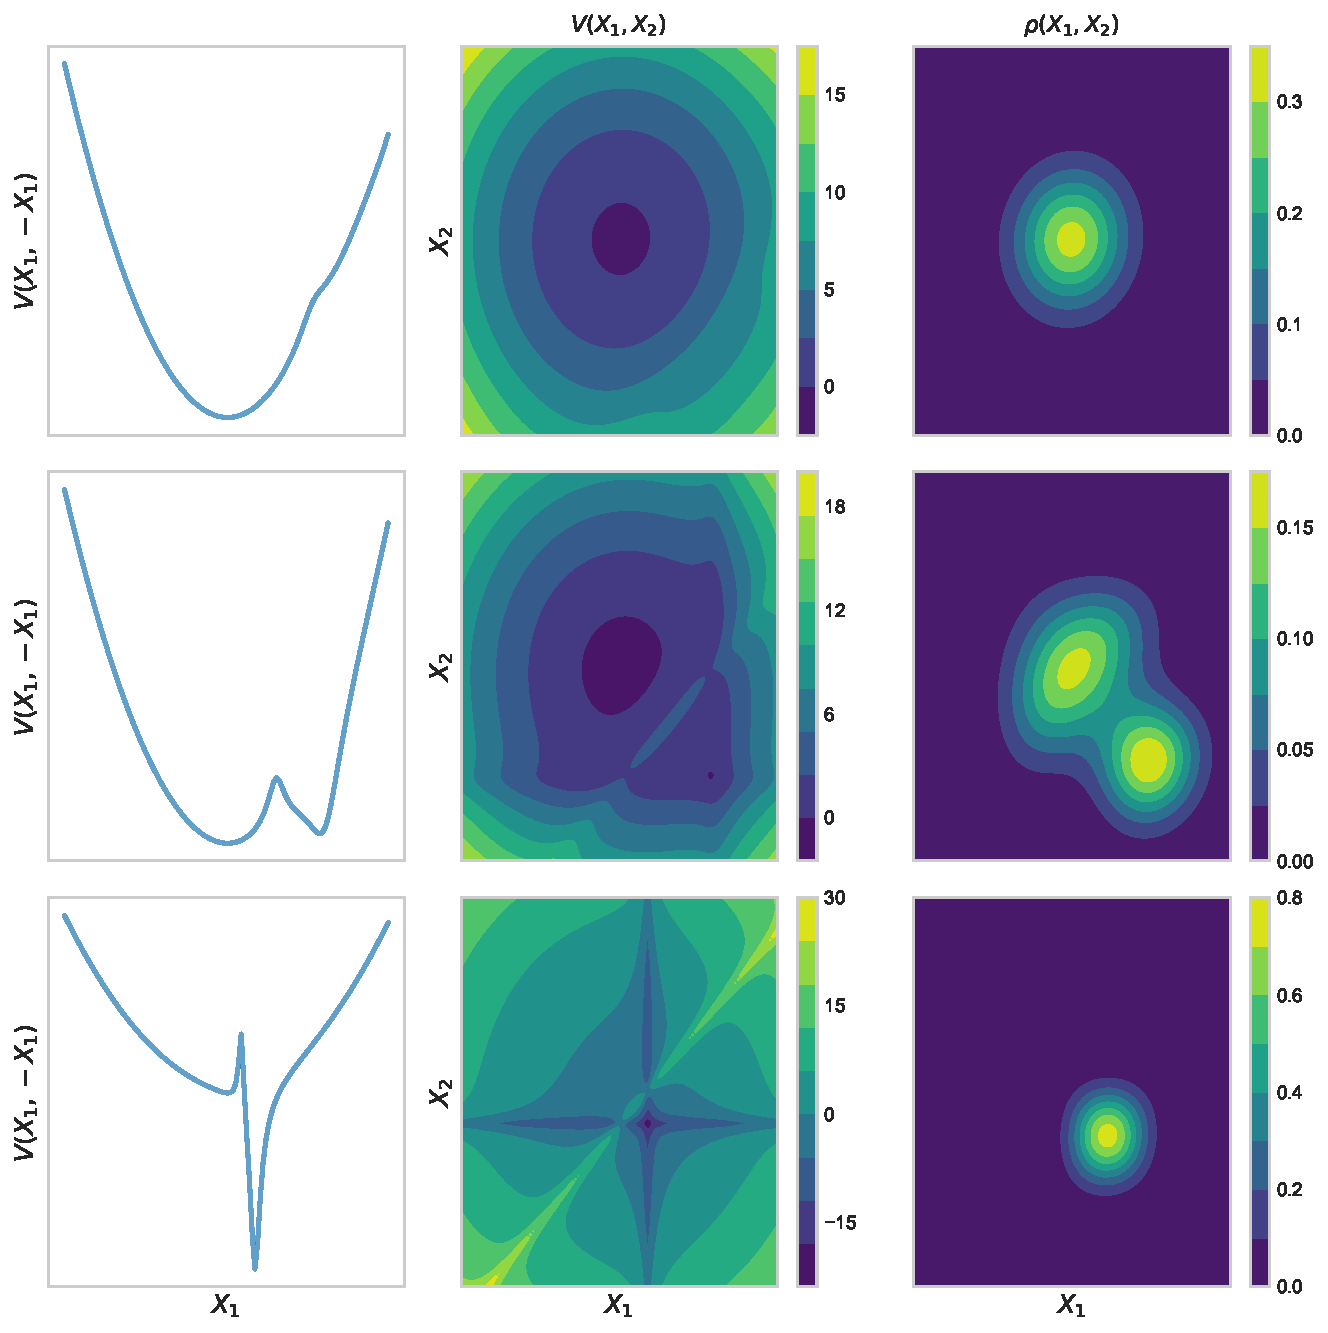
\includegraphics[scale=0.85]{figures/classical_potential_small_angle.pdf}
        %\end{subfigure}
        \caption{\label{fig:classical_potential_small_angle}\textbf{From top to bottom:} $d=3.16$: QDOs are far apart, $d=1.75$: Maximal interaction between the QDOs, $d=0.51$: deep in the bound state. \textbf{From left to right:} joint position quadrature distribution of the two drudons, classical potential energy $V(X_1,X_2) = V_\text{Coul}(X_1,X_2) + (X_1^2 + X_2^2) /2$, diagonal section of the joint distribution and of the potential. Tunneling between the quadratic and Coulomb wells is maximal at the intermediate interatomic distance as can be seen from the bimodal joint distribution, and the neat appearance of two local vacua in the classical potential. This figure corresponds to the small angle $\theta=0.17$.}
    \end{figure*}

\paragraph*{Ground state wavefunction and entanglement entropy}

    \begin{figure*}
        %\hspace{1.25cm}
        %\begin{subfigure}
        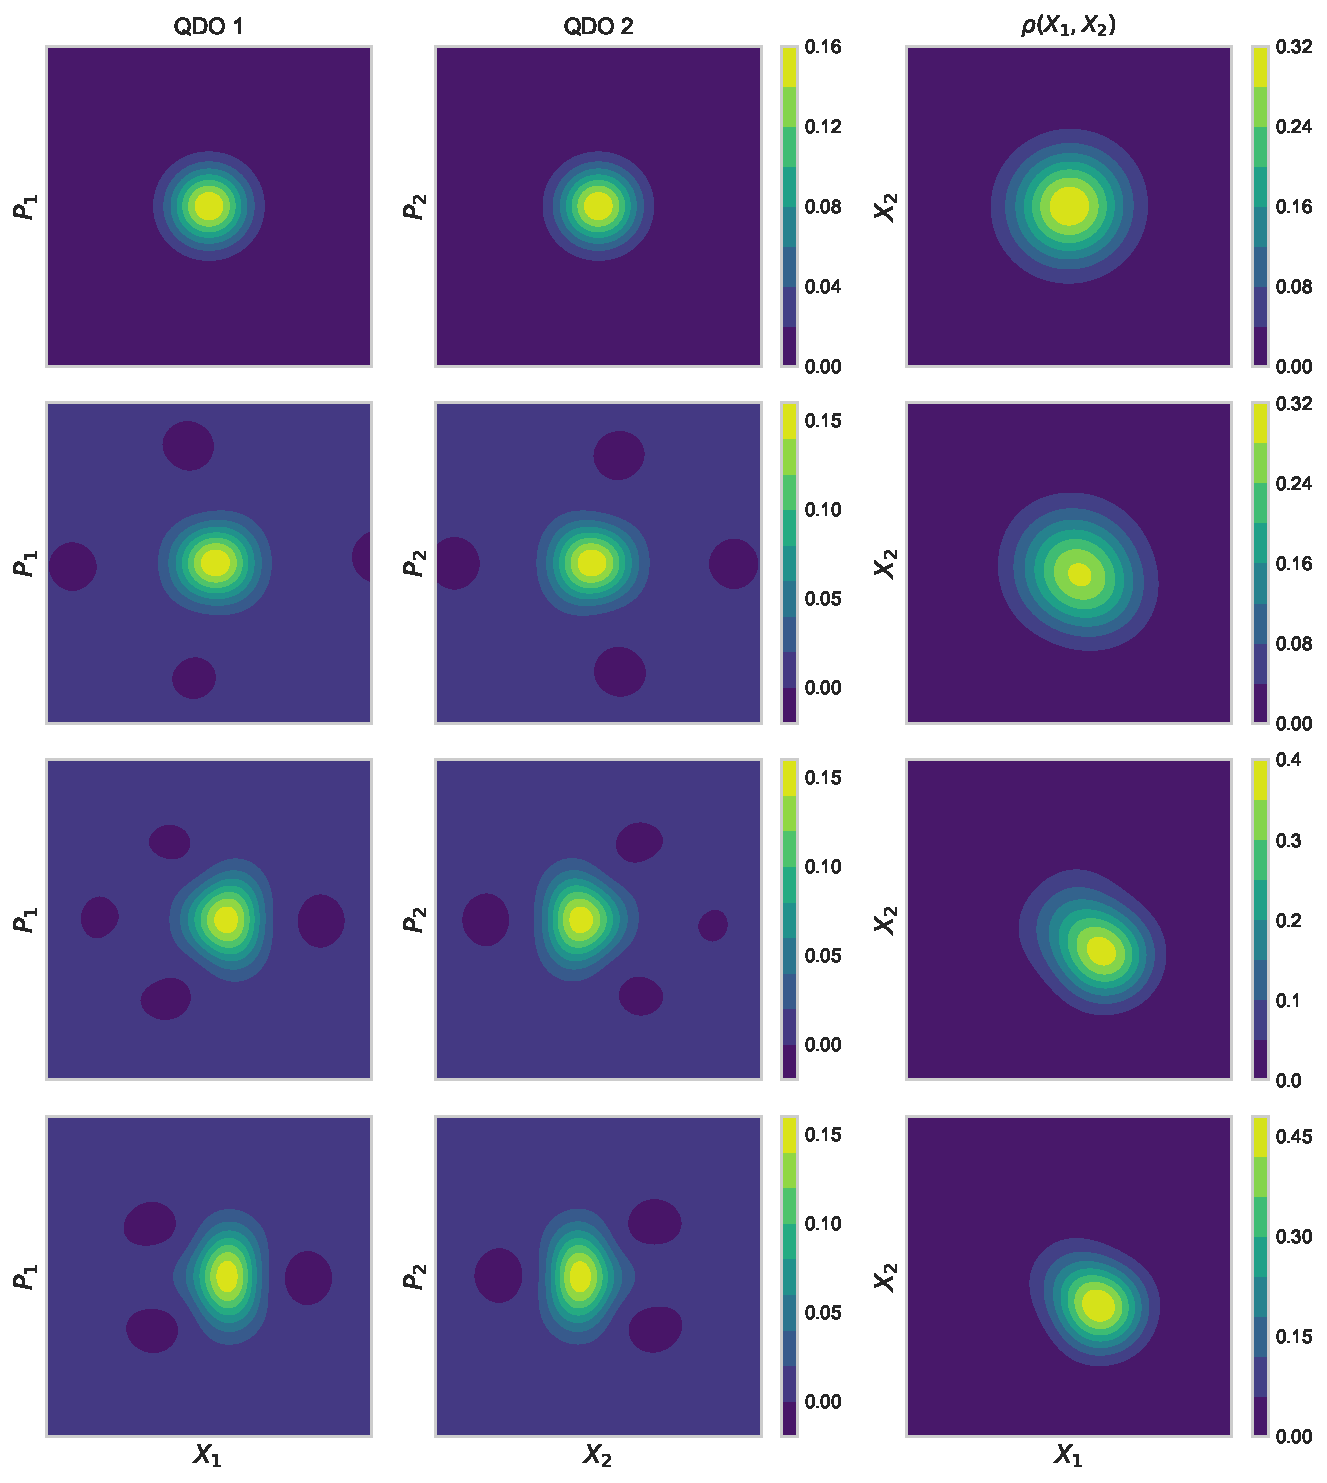
\includegraphics[scale=0.75]{figures/wigners_joint.pdf}
        %\end{subfigure}
        \caption{\label{fig:wigners_joint}\textbf{From top to bottom:} $d=3.16$: QDOs are far apart, $d=1.36$: QDOs start feeling each other, $d=0.82$: entanglement entropy is maximal, $d=0.54$: deep in the bound state. \textbf{From left to right:} Wigner distribution of the left QDO, Wigner distribution of the right QDO, joint position quadrature distribution of the two drudons.}
    \end{figure*}

    In order to gain more intuition about the information possessed about one part of our bipartite system concerning the other part, let us introduce the partial density matrix associated to $\text{QDO}_1$. The total state of the system, we recall, is expressed in the Fock basis as the pure state:
    \begin{equation*}
        |\psi\rangle = \sum_{n_1,n_{2}=0}^\infty \alpha_{n_1n_2}|n_1\rangle\otimes|n_2\rangle\,.
    \end{equation*}
    This state is directly accessible when using the simulator, and can be obtained on a genuine hardware by state tomography techniques \cite{Lvovsky:2009zz}. Given the pure state describing the full system, the density matrix of the system is simply given by:
    \begin{equation*}
        \rho = \sum_{\substack{n_1,n_2 \\ m_1,m_2}} \alpha^*_{m_1m_2}\alpha_{n_1n_2}|n_1\rangle\langle m_1|\otimes|n_2\rangle\langle m_2|\,.
    \end{equation*}
    The partial trace associated to $\text{QDO}_1$ is therefore given by:
    \begin{equation*}
        \rho_1 = \sum_{n, m, l} \alpha^*_{ml}\alpha_{nl}\,|n\rangle\langle m|\,.
    \end{equation*}
    Since the state of the total system is pure, $\text{QDO}_2$ can be interpreted as purifying the system composed solely of $\text{QDO}_1$. The two QDOs therefore have identical von Neumann entropy $S(\rho_1)$, the entanglement entropy. The quantum mutual information of the system is therefore given by
    \begin{equation*}
        I(1:2) = S(\rho_1) + S(\rho_2) - S(\rho) = 2S(\rho_1) \,,
    \end{equation*}
    with the von Neumann entropy being defined as
    \begin{equation*}
        S(\rho) = -\text{Tr}\left[\rho\log\rho\right]\,.
    \end{equation*}
    The profile of the quantum mutual information for different values of the angle $\theta$ as a function of the interatomic distance is provided in fig. \ref{fig:entropy_correlation} (top).
    \begin{figure}[h]
        \hspace{-0.4cm}
        \centering
        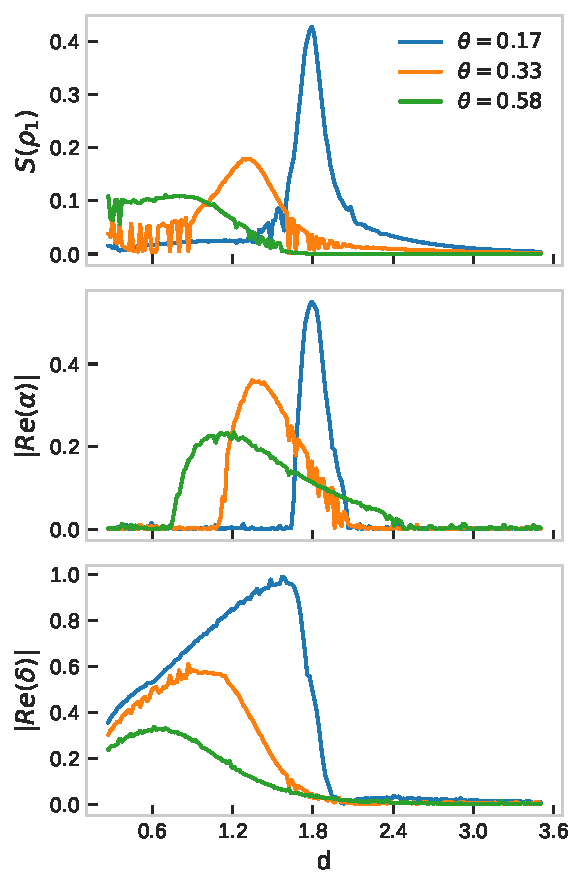
\includegraphics[scale=0.9]{figures/alpha_delta_rho.pdf}
        \caption{\label{fig:entropy_correlation}\textbf{On the top.} Entanglement entropy as a function of the distance $d$ between QDOs for multiple values of $\theta$. \textbf{In the middle.} Absolute value of $\mathrm{Re}\left(\alpha\right)$ resulting from the fitted displaced cat ansatz. \textbf{On the bottom.} Absolute value of $\mathrm{Re}\left(\delta\right)$ resulting from the fitted displaced cat ansatz.}
    \end{figure}
    In this figure we can see how for small values of $theta$ the entanglement entropy presents a sharp peak which gradually turns into a plateau-like behaviour as $theta$ increases ($\theta = 0.58$ is the highest angle for which a peak is found). A fit of the entanglement entropy for angle $\theta = 0.58$ is provided in fig. \ref{fig:entropy_correlation2} (top).

    This finding, together with the behaviour of the joint probability reported in fig. \ref{fig:wigners_joint}, gives us an intuition of what happens to the ground state of the system along the binding process. For $d\rightarrow \infty$ the two QDOs will not interact and hence the natural state for them will be the vacuum state $\ket{0}\ket{0}$ (ground state of independent harmonic oscillators). On the other hand when $d \sim d_{\mathrm{bonding}}$ we see that the system is shifted towards an antisymmetric configuration where $\langle X_1\rangle -\langle X_2\rangle$ and $\langle P_1\rangle = \langle P_2\rangle = 0$, which can be approximated by the bipartite coherent state $\ket{\alpha}\ket{-\alpha}$ with $\alpha = \tilde{X}$. In the transition region instead the system will pass through a strongly entangled state (hence the peak in von Neumann entropy), which is reflected in the joint probability as a delocalized between the two configurations we just mentioned. This is naturally represented as a superposition of the form
    \begin{equation*}
        \frac{1}{\mathcal{N}}\left(\ket{0}\otimes\ket{0} + \ket{\alpha}\otimes\ket{-\alpha}\right),
    \end{equation*}
    where $\mathcal{N}$ is a normalization factor, which is nothing but a displaced entangled cat state, namely:
    \begin{equation*}
        \frac{1}{\mathcal{N}}\,\hat{D}_{\frac{\alpha}{2}}\otimes\hat{D}_{-\frac{\alpha}{2}}\left(\left|-\frac{\alpha}{2}\right\rangle\otimes\left|\frac{\alpha}{2}\right\rangle + \left|\frac{\alpha}{2}\right\rangle\otimes\left|-\frac{\alpha}{2}\right\rangle\right),
    \end{equation*}
    where $\hat{D}_{t} = e^{t\hat{a}^{\dagger} - t^{*}\hat{a}}$ is the dispacement operator.

    To further prove that our intuition/approximation is indeed correct, we define and pointwise fit (for each value of the interactomic distance) the following ansatz to our ground state wavefunction $\psi(\theta, d)$:
    \begin{equation*}
    \begin{split}
        \ket{\zeta(\alpha, \delta)} = \frac{1}{\mathcal N}(&\ket{\alpha-\delta}\otimes\ket{-\alpha + \delta} \\
        &+ \ket{-\alpha-\delta}\otimes\ket{\alpha + \delta}).
    \end{split}
    \end{equation*}
    by maximizing the state fidelity:
    \begin{equation*}
        \mathcal{F}_{\theta, d}(\alpha, \delta) = |\braket{\zeta(\alpha, \delta)}{\psi(\theta, d)}|^2.
    \end{equation*}
    \begin{figure}[h]
        \centering
        \subfloat{%
          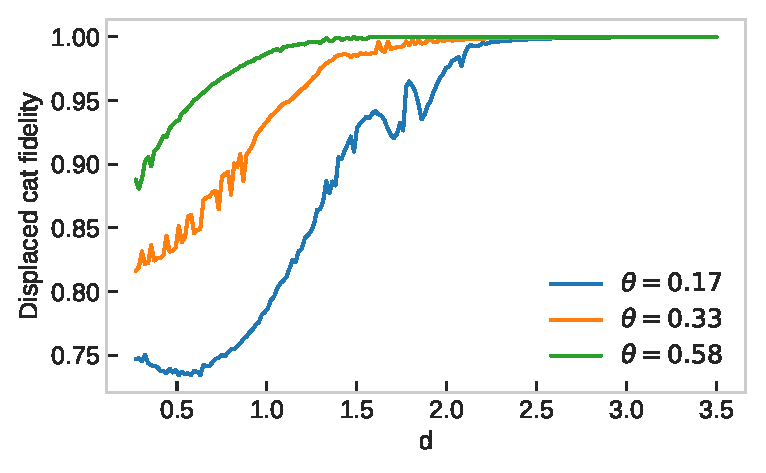
\includegraphics[clip,width=\columnwidth]{figures/fidelities.pdf}%
        }
        \vspace{-3ex}
        \subfloat{%
          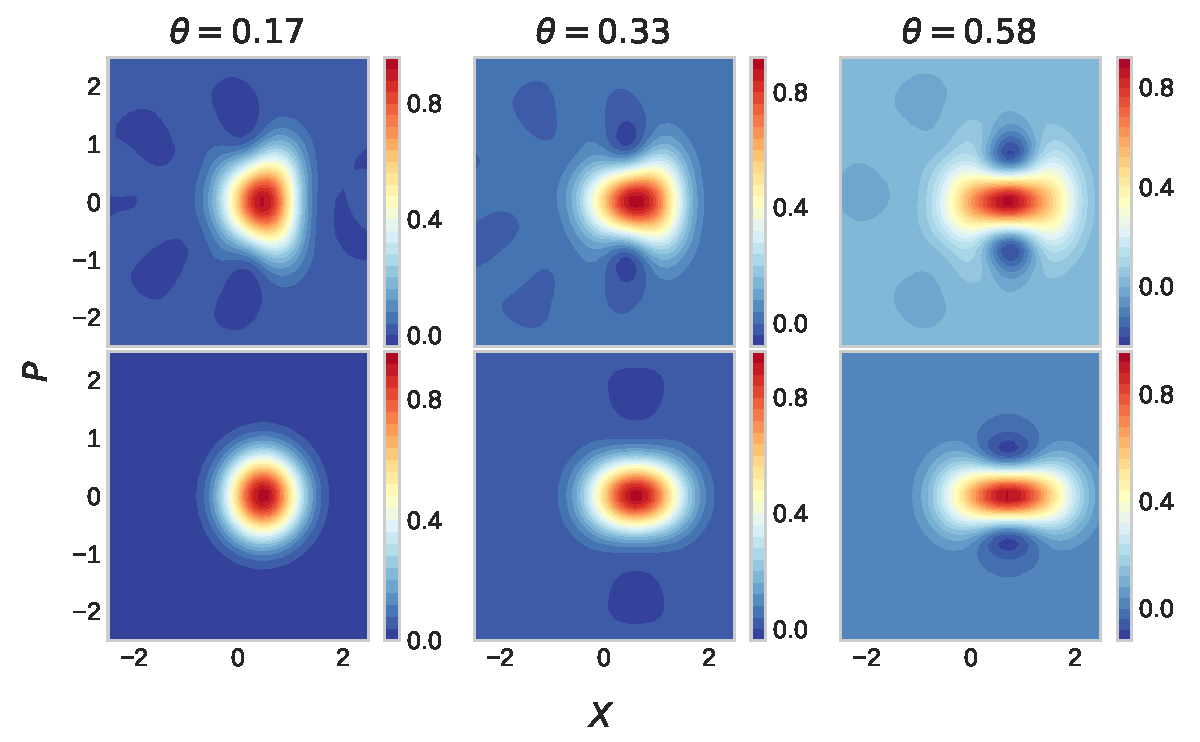
\includegraphics[clip,width=1.\columnwidth]{figures/ground_cat_wigner.pdf}%
        }
        \caption{\label{fig:fidecats}\textbf{On the top.} Fidelity results for the fit of the ansatz $\ket{\zeta(\alpha, \delta)}$ at different values of $\theta$. \textbf{On the bottom.} Comparison between the states of the system on the entropy peaks (top) and the fitted ansatz in the same point (bottom). We plot the Wigner function sliced along the mainfold $(X = X_1 = -X_2, P = P_1 = -P_2$).}
    \end{figure}
    In fig. \ref{fig:fidecats} (top) we report the obtained behaviour for $\mathcal{F}_{\theta, d}$. Although there is a deterioration in the fit for decreasing values of theta, our minimal ansatz can indeed approximate the ground state of the system up to a good degree for all the considered thetas: it manages to capture the bonding mechanism (states for which there is an entropy peak) with $\mathcal{F}\sim 0.96$. A comparison at the level of Wigner functions between the original and fitted states for those bonding points is reported in fig. \ref{fig:fidecats} (bottom). Moreover, by looking at the behaviour of the fitted values of $\alpha$ and $\delta$ together with entanglement entropy in fig. \ref{fig:entropy_correlation}, we can see how indeed the behaviour of the system follows our intuition: for $d\rightarrow\infty$ we have $(\alpha, \delta) = (0,0)$ and entanglement entropy close to zero, for $d\sim d_{bonding}$ we have that $\alpha \sim 0$ and $\delta\neq 0$ corrisponging to an original state with low (alothough non-zero) value of entanglement entropy, and for the transition region we see that the peak of entanglement entropy matches almost perfectly the peak in the value of $\alpha$. Let us mention that the production of cat states typically involves the use of Kerr and squeezing gates \cite{puri2017engineering, grimm2019kerr}, both of which being present in our quantum neural network architecture, Kerr gates being the source of non-Gaussianity and entanglement of the ansatz.

    Given the joint position quadrature density, another interesting quantity to consider is the quantum correlation between the position quadrature of the two QDOs, which appears to be highly correlated to the behavior of the entanglement entropy. Denoting again by angular brackets the expectation of an observable in the ground state, we define the correlation coefficient $C(X_1, X_2)$ by:
    \begin{equation*}
        C(X_1, X_2) = \frac{\langle X_1X_2\rangle - \langle X_1\rangle\langle X_2\rangle}{\sqrt{\langle X_1^2\rangle - \langle X_1\rangle^2}\sqrt{\langle X_2^2\rangle - \langle X_2\rangle^2}}\,.
    \end{equation*}

    \begin{figure}
        %\hspace{1.25cm}
        %\begin{subfigure}
        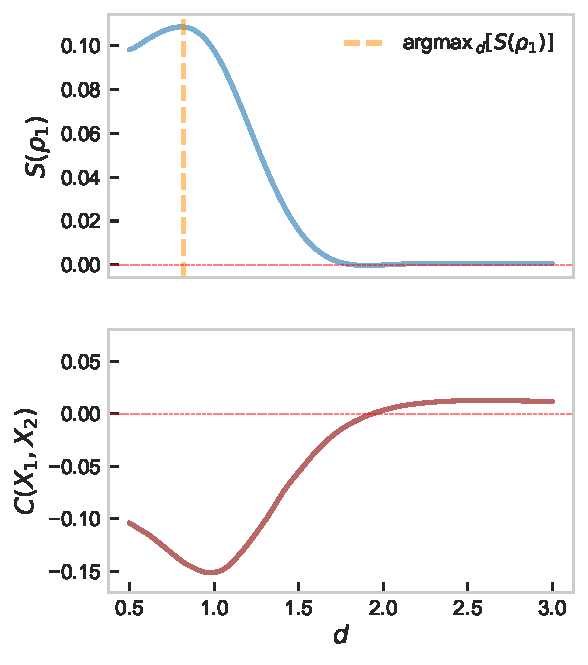
\includegraphics[scale=0.7]{figures/entropy_correlation.pdf}
        %\end{subfigure}
    \caption{\label{fig:entropy_correlation2}\textbf{On the top.} Entanglement entropy vs. interatomic distance. \textbf{On the bottom.} Position quadratures correlation coefficient vs. interatomic distance. Both curves correspond to the model at angle $\theta=0.58$.}
    \end{figure}

    %\begin{figure}
    %    %\hspace{1.25cm}
    %    %\begin{subfigure}
    %    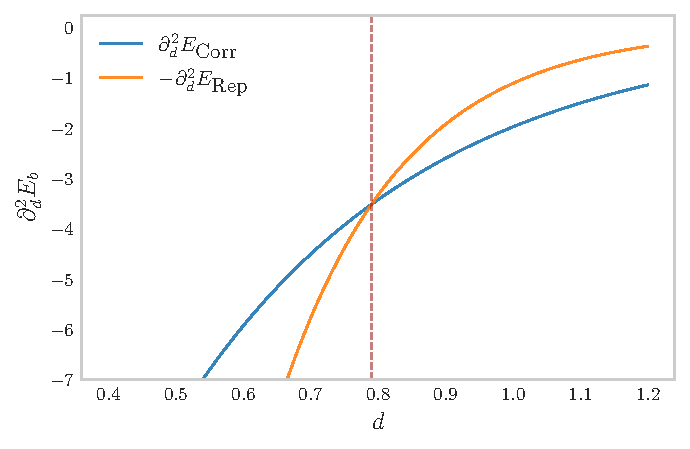
\includegraphics[scale=0.75]{figures/repulsion_vs_correlation_2nd_derivative.pdf}
    %    %\end{subfigure}
    %    \caption{\label{fig:second_derivatives}Competition between correlation and Coulomb repulsion energies for the model at $\theta=0.58$. Their second derivatives intersect at the inflexion point of the binding curve.}
    %\end{figure}

    Even though we do not have a neat theoretical understanding of it, we note that the maximum of the entanglement entropy, as well as the minimum of the correlation coefficient, converges towards the inflexion point of the the binding energy curve as the value of $\theta$ increasing. A zeroth order line of argument could be the following: the binding energy is composed of a Coulomb repulsion and an attractive correlation energy contribution:
    \begin{equation*}
        E(d)=E_\text{Rep}(d)+E_\text{Corr}(d)
    \end{equation*}
    The inflexion point $d_\star$, which in terms of the Morse fit (\ref{eq:morse_fit}) is located at $d_\star = d_b + \log(2)s$,
    %\begin{equation*}
    %    \frac{\partial^2 E_\text{Rep}}{\partial d^2}(d_\star) = -\frac{\partial^2 E_\text{Corr}}{\partial d^2}(d_\star)\,,
    %\end{equation*}
    can be interpreted as the transition between a large distance regime in which it is beneficial for the system to increase correlation in order to lower its ground state energy, and a short range regime in which the Coulomb repulsion becomes dominant. Further understanding of this phenomenon in the language of phase transitions would be very interesting, but is left for a more theoretical investigation.



\paragraph*{Conclusion}

    In this letter, we showed that continuous variables photonics quantum computing is particularly adapted to the study of the full-Coulomb Many Body Dispersion model, the fundamental degrees of freedom of the latter being bosonic in nature. Beyond standing as a proof-of-concept that NISQ algorithms can be successfully applied to quantum chemistry problems beyond the usual approach using the second quantized formulation of the electronic structure problem for small molecules, we observed that the standard QDO toy model for Many Body Dispersion can be further simplified by reducing it to a single effective spatial dimension (at least for the two-QDO system), together with a reparameterization of the QDO parameters.
    \newline

\paragraph*{acknowledgments}

    We would like to thank Dahvyd Wing and Kyunghoon Han for helpful discussions.
    \newline

\paragraph*{Code Availability}

The reader will find an open source python code accompanying this paper at the following \href{https://github.com/MatthieuSarkis/qdo}{github repository}.

\appendix

%\nocite{*}
\bibliographystyle{IEEEtran}
\bibliography{bibliography}

\end{document}


%%%%%%%%%%%%%%%%%%%%%%%%%%%%%%%%%%%%%%%%%%%%%%%%%%%%
%%%%%%%%%%% UNUSED CODE %%%%%%%%%%%%%%%%%%%%%%%%%%%%
%%%%%%%%%%%%%%%%%%%%%%%%%%%%%%%%%%%%%%%%%%%%%%%%%%%%


Let us give here the expression for the multipolar potential up to quartic order:
        \begin{align}
            V_0(\bm{x} _i, \bm{x} _j) &= q_iq_j\frac{x_ix_j + y_iy_j - z_iz_j}{r_{ij}^3}\\
            V_1(\bm{x} _i, \bm{x} _j) &= \frac{q_iq_j}{2r_{ij}^4}\big(-3  x_i ^2  z_j -6  x_i   x_j   z_i +6  x_i   x_j   z_j +3  x_j ^2  z_i\nonumber\\
            & -3  y_i ^2  z_j -6  y_i   y_j   z_i +6  y_i   y_j   z_j +3  y_j ^2  z_i\nonumber\\
            & +6  z_i ^2  z_j -6  z_i   z_j ^2\big)\\
            V_2(\bm{x} _i, \bm{x} _j) &= \frac{q_iq_j}{2 r_{ij}^4}\big(-6  x_i ^3  x_j +9  x_i ^2  x_j ^2-6  x_i ^2  y_i   y_j +3  x_i ^2  y_j ^2\nonumber\\
            &+24  x_i ^2  z_i   z_j -12  x_i ^2  z_j ^2-6  x_i   x_j ^3-6  x_i   x_j   y_i ^2\nonumber\\
            &+12  x_i   x_j   y_i   y_j -6  x_i   x_j   y_j ^2+24  x_i   x_j   z_i ^2\nonumber\\
            &-48  x_i   x_j   z_i   z_j +24  x_i   x_j   z_j ^2+3  x_j ^2  y_i ^2-6  x_j ^2  y_i   y_j \nonumber\\
            &-12  x_j ^2  z_i ^2+24  x_j ^2  z_i   z_j -6  y_i ^3  y_j +9  y_i ^2  y_j ^2\nonumber\\
            &+24  y_i ^2  z_i   z_j -12  y_i ^2  z_j ^2-6  y_i   y_j ^3+24  y_i   y_j   z_i ^2\nonumber\\
            &-48  y_i   y_j   z_i   z_j +24  y_i   y_j   z_j ^2-12  y_j ^2  z_i ^2+24  y_j ^2  z_i   z_j \nonumber\\
            &-16  z_i ^3  z_j +24  z_i ^2  z_j ^2-16  z_i   z_j ^3\big)
        \end{align}



        \begin{equation}
            \begin{split}
                &V_0(x_i, x_j) = q_iq_j\frac{x_ix_j}{r_{ij}^3}\times\\
                &\times\begin{cases}
                    1-3\cos^2\theta, & \text{generic case} \\
                    -2, & \text{parallel case} \\
                    1, & \text{perpendicular case} \\
                    -\frac{1}{2}, & \text{oblique case} \\
                    -2-6\epsilon, & \text{regularized case}
                \end{cases}
            \end{split}
            \end{equation}
            The next terms in the multipolar expansion are:
            \begin{equation}
            \begin{split}
                &V_1(x_i, x_j) = q_iq_j\frac{x_ix_j(x_i-x_j)}{r_{ij}^4}\times\\
                &\times\begin{cases}
                    \frac{3\cos\theta(-3+5\cos^2\theta)}{2}, & \text{generic case} \\
                    3, & \text{parallel case} \\
                    0, & \text{perpendicular case} \\
                    -\frac{3}{4\sqrt 2}, & \text{oblique case} \\
                    3+18\epsilon, & \text{regularized case}
                \end{cases}
            \end{split}
            \end{equation}
            \begin{equation}
                \begin{split}
                    &V_2(x_i, x_j) = q_iq_j\frac{x_ix_j(2x_i^2-3x_ix_j+2x_j^2)}{r_{ij}^5}\times\\
                    &\times
                    \begin{cases}
                        -\frac{3-30\cos^2\theta+35\cos^4\theta}{4}, & \text{generic case} \\
                        -2, & \text{parallel case} \\
                        -\frac{3}{4}, & \text{perpendicular case} \\
                        \frac{13}{16}, & \text{oblique case} \\
                        -2-20\epsilon, & \text{regularized case}
                    \end{cases}
                \end{split}
            \end{equation}

            \subsection{12 different models}

            For the simulation, we will restrict the system to two QDOs. Depending on the space dimensionality (1d oblique, 1d parallel, 1d perpendicular, 3d) and the choice of potential (quadratic, quartic, Coulomb), we therefore have 12 models to try and study, gathered in table (\ref{tab:models}).
            \begin{table}[ht!]
            \caption{\label{tab:models} The twelve models}
            \begin{ruledtabular}
            \begin{tabular}{c|cccc}
                \diagbox[height=1.8\line]{\textsc{pot}}{\textsc{dim}}& 1d oblique & 1d parallel & 1d perpendicular & 3d \\
                \hline\\[-0.95em]
                \textsc{quad} & $H_{(1,0)}$ & $H_{(1,1)}$ & $H_{(1,2)}$ & $H_{(1,3)}$ \\
                \textsc{quart} & $H_{(2,0)}$ & $H_{(2,1)}$ & $H_{(2,2)}$ & $H_{(2,3)}$\\
                \textsc{Coulomb} & $H_{(3,0)}$ & $H_{(3,1)}$ & $H_{(3,2)}$ & $H$ \\
            \end{tabular}
            \end{ruledtabular}
            \end{table}

            The space regularized model Coulomb potential reads
            \begin{equation}
            \begin{split}
                &\frac{V_\text{Coul}^\epsilon(x_i, x_j)}{q_iq_j} = \frac{1}{r_{ij}} - \frac{1}{\sqrt{r_{ij}^2+2r_{ij}(1+\epsilon) x_i+x_i^2}} \\
                &- \frac{1}{\sqrt{r_{ij}^2-2r_{ij}(1+\epsilon) x_j+x_j^2}} \\
                &+\frac{1}{\sqrt{r_{ij}^2 - 2r_{ij}(1+\epsilon) (x_j-x_i) + (x_j-x_i)^2}}\,.
            \end{split}
            \end{equation}

            In terms of components, the full Coulomb potential reads:
            \begin{equation}
            \mathclap{
            \begin{split}
                &\frac{V_\text{Coul}(\bm{x} _i, \bm{x} _j)}{q_iq_j} = \frac{1}{r_{ij}} - \frac{1}{\sqrt{r_{ij}^2 + x_i^2+y_i^2+z_i^2+2rz_i}} \\
                &- \frac{1}{\sqrt{r_{ij}^2 + x_j^2+y_j^2+z_j^2-2r_{ij}z_j}} \\
                &+\frac{1}{\sqrt{r_{ij}^2 + (x_j-x_i)^2+(y_j-y_i)^2+(z_j-z_i)^2-2r_{ij}(z_j-z_i)}}
            \end{split}
            }
            \end{equation}

            For the full Coulomb potential, assuming that the drudons are constrained to move along an axis, we get the following expressions:
            \begin{equation}
            \begin{split}
                \frac{V_\text{Coul}^\perp(x_1, x_2)}{q_1q_2} = &\ \frac{1}{r_{12}} - \frac{1}{\sqrt{r_{12}^2+x_1^2}} - \frac{1}{\sqrt{r_{12}^2+x_2^2}} \\
                &+\frac{1}{\sqrt{r_{12}^2 + (x_2-x_1)^2}}
            \end{split}
            \end{equation}
            in the case where the drudons move perpendicular to the axis joining the two nuclei, and
            \begin{equation*}
            \mathclap{
                \frac{V_\text{Coul}^{||}(x_1, x_2)}{q_1q_2} = \frac{1}{r_{12}} - \frac{1}{|r_{12}+x_1|} - \frac{1}{|r_{12}-x_2|} + \frac{1}{|r_{12}+x_1-x_2|}
            }
            \end{equation*}
            in the case where they move parallel to the latter.


            \begin{equation}
                |\psi(\omega)\rangle = \sum_{n_1,\dots,n_{2K}=0}^\infty \alpha_{n_1\dots n_{2K}}|n_1\rangle\otimes\dots\otimes|n_{2K}\rangle\,.
            \end{equation}
            The modes labeled by $(n_1,\dots,n_K)$ correspond to $\text{QDO}_1$, while the modes $(n_{K+1},\dots,n_{2K})$ are attached to $\text{QDO}_2$.
            The amplitude of a specific tuple of the quadratures $(X_1,\dots, X_{K})$ is therefore given by:
            \begin{equation*}
            \mathclap{
                \langle X_1,\dots,X_{2K}|\psi\rangle = \sum_{n_1,\dots,n_{2K}=0}^\infty \alpha_{n_1\dots n_{2K}}\prod_{i=1}^{2K}\frac{e^{-\sum_{i=1}^{2K}\frac{X_i^2}{2}}H_{n_i}(X_i)}{\sqrt{\pi^{1/2}2^{n_i}n_i!}}\,,
            }
            \end{equation*}
            in terms of the Hermite polynomials. The joint law of the quadratures in the state $|\psi\rangle$ is therefore given by
            \begin{equation}
            \begin{split}
                \rho(X_1,\dots,X_{2K}) &= \sum_{\substack{n_1,\dots,n_{2K} \\ m_1,\dots,m_{2K}}} \alpha_{n_1\dots n_{2K}}\alpha^*_{m_1\dots m_{2K}}\\
                &\times\prod_{i=1}^{2K}\frac{e^{-X_i^2}H_{n_i}(X_i)H_{m_i}(X_i)}{\sqrt{\pi^{1/2}2^{n_i}n_i!}\sqrt{\pi^{1/2}2^{m_i}m_i!}}
            \end{split}
            \end{equation}
            After extracting as well the mean photon numbers $\langle n_{i,\alpha}\rangle$, one obtains $\langle H\rangle$.

            \begin{algorithm}
                \caption{Computation of the loss}\label{alg:loss_computation}
                    \textbf{Parameters:} $M\in\mathbb N$

                    \KwResult{Value of the loss $\mathcal C$}\

                    Initialize $\mathcal C \gets 0$\;
                    Get the position quadratures distribution with alg. (\ref{alg:statistics_computation})\;
                    Get the photon numbers distribution with alg. (\ref{alg:statistics_computation})\;
                    Compute the loss $\mathcal C$ using eq. (\ref{eq:loss})\;
                    \textbf{return} $\mathcal C$.
            \end{algorithm}

            \begin{equation}
                |\psi\rangle = \sum_{n_1,\dots,n_{2K}=0}^\infty \alpha_{n_1\dots n_{2K}}|n_1\rangle\otimes\dots\otimes|n_{2K}\rangle\,,
            \end{equation}
            leading to the following expression for the density matrix:
            \begin{equation*}
            \mathclap{
                \rho = \sum_{\substack{n_1,\dots,n_{2K} \\ m_1,\dots,m_{2K}}} \alpha^*_{m_1\dots m_{2K}}\alpha_{n_1\dots n_{2K}}|n_1\rangle\langle m_1|\otimes\dots\otimes|n_{2K}\rangle\langle m_{2K}|\,.
            }
            \end{equation*}
            The partial trace associated to $\text{QDO}_1$ is therefore given by:
            \begin{equation}
            \begin{split}
                \rho_1 = \sum_{\substack{n_1,\dots,n_{K} \\ m_1,\dots,m_{K} \\ l_1,\dots,l_{K}}}& \alpha^*_{m_1\dots m_{K}l_1,\dots,l_{K}}\alpha_{n_1\dots n_{K}l_1,\dots,l_{K}}\\
                &|n_1\rangle\langle m_1|\otimes\dots\otimes|n_{K}\rangle\langle m_{K}|\,.
            \end{split}
            \end{equation}